\documentclass[a4paper, 12pt]{article}
\usepackage{graphicx}
\usepackage{amssymb, amsfonts, amsmath, amsthm}
\usepackage[margin=1in]{geometry}
\usepackage{enumitem}
\usepackage{array}
\usepackage{fancyhdr}
\usepackage{tikz}
\usepackage{parskip}
\usepackage{float}
\usetikzlibrary{automata, positioning, arrows}
\usetikzlibrary{graphs}

\setlength{\headheight}{14.49998pt}

\tikzset {
    ->,
    >=stealth',
    node distance=3cm,
    every state/.style={thick, fill=gray!10},
    initial text = $ $
}

\makeatletter
\renewenvironment{proof}[1][\proofname]{\par
%  \pushQED{\qed}% <--- remove the QED business
  \normalfont \topsep6\p@\@plus6\p@\relax
  \trivlist
  \item[\hskip\labelsep
        \itshape
    #1\@addpunct{.}]\ignorespaces
}{%
%  \popQED% <--- remove the QED business
  \endtrivlist\@endpefalse
}
\renewcommand\qedhere{} % to ensure code portability
\makeatother

\pagestyle{fancy}
\fancyhead[l]{SECJ3203}
\fancyhead[c]{Tutorial 5}
\fancyhead[r]{23 April 2024}

\title{Tutorial 3 & 4}
\date{}
\author{}

\renewcommand{\proofname}{Solution:}

\begin{document}
    \begin{enumerate}
        \item Let \(\Sigma = \{a, b\}\). For the language, $L$ that are defined by each of the following grammars
        \begin{enumerate}[label=(\roman{*})]
            \item \(S \to aS \mid Sb \mid \varepsilon\)
            \item \(S \to aS \mid bS \mid \varepsilon\)
        \end{enumerate}

        Do each of the following:
        \begin{enumerate}

            \item List TWO strings that are in $L$.
            \begin{proof}
                $ab, abb$
            \end{proof}

            \item List TWO strings that are not in $L$.
            \begin{proof}
                There are no strings that are not in $L$.
            \end{proof}

            \item Describe $L$ consisely. You can use regular expressions or set theoretic expressions.
            \begin{proof}
                The grammar of the language $L$ can be described as \(G = (V, \Sigma, P, S)\), where \(V = \{a, b, S\}\), \(\Sigma=\{0, 1\}\), starting symbol $S$ and productions $P$ described as above.

                The language generated by the grammar, $L$ can be described with the regular expression $L(G) = (a+b)^*$.
            \end{proof}

            \item State whether $L$ is a regular language or not.
            \begin{proof}
                $L$ is a regular language.
            \end{proof}
        \end{enumerate}

        \item Draw a FA diagram for each of the regular grammar below.
        \begin{enumerate}
            % -------
            \item \( \begin{aligned}[t]
                S &\to aS \mid bA \mid \lambda \\
                A &\to bA \mid \lambda
            \end{aligned} \)

            \begin{proof}
                \leavevmode\par

                \begin{center}
                    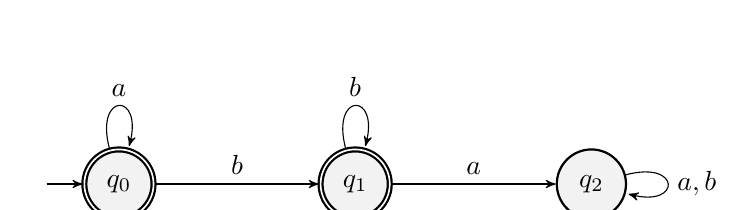
\begin{tikzpicture}
                        \node[state, initial, accepting] (q0) {$q_0$};
                        \node[state, accepting, right of=q0] (q1) {$q_1$};
                        \node[state, right of=q1] (q2) {$q_2$};

                        \draw 
                        (q0) edge[loop above] node{$a$} (q0)
                        (q0) edge[above] node{$b$} (q1)
                        (q1) edge[loop above] node{$b$} (q1)
                        (q1) edge[above] node{$a$} (q2)
                        (q2) edge[loop right] node{$a, b$} (q2);
                    \end{tikzpicture}
                \end{center}

            \end{proof}
            % -------

            % -------
            \item \( \begin{aligned}[t]
                S &\to aS \mid bA \mid \lambda \\
                A &\to aS \mid bA \mid \lambda
            \end{aligned} \)

            \begin{proof}
                \leavevmode \par

                \begin{center}
                    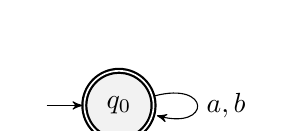
\begin{tikzpicture}
                        \node[state, initial, accepting] (q0) {$q_0$};

                        \draw
                        (q0) edge[loop right] node{$a, b$} (q0);
                    \end{tikzpicture}
                \end{center}
            \end{proof}
            % -------

            \newpage

            % -------
            \item \( \begin{aligned}[t]
                S &\to aA \mid bS \\
                A &\to aB \mid bS \\
                B &\to aB \mid bB \mid \lambda
            \end{aligned} \)

            \begin{proof}
                \leavevmode \par

                \begin{center}
                    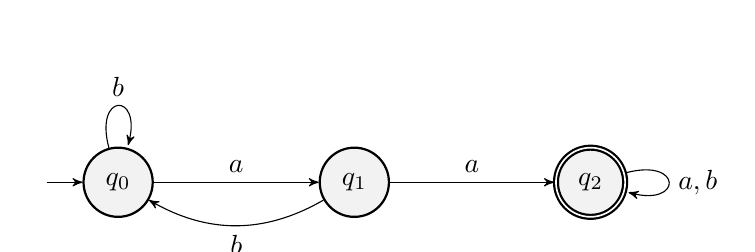
\begin{tikzpicture}
                        \node[state, initial] (q0) {$q_0$};
                        \node[state, right of=q0] (q1) {$q_1$};
                        \node[state, accepting, right of=q1] (q2) {$q_2$};

                        \draw
                        (q0) edge[loop above] node{$b$} (q0)
                        (q0) edge[above] node{$a$} (q1)
                        (q1) edge[above] node{$a$} (q2)
                        (q1) edge[bend left] node[below=0]{$b$} (q0)
                        (q2) edge[loop right] node{$a, b$} (q2);
                        
                    \end{tikzpicture}
                \end{center}
            \end{proof}
            % -------

            % -------
            \item \( \begin{aligned}[t]
                S &\to aA \mid bS \\
                A &\to aA \mid bS \mid \lambda
            \end{aligned} \)

            \begin{proof}
                \leavevmode \par

                \begin{center}
                    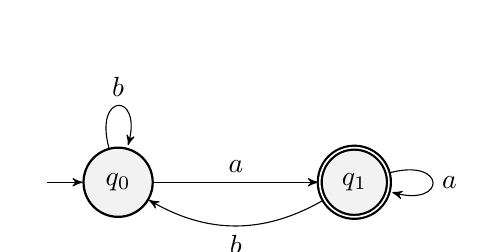
\begin{tikzpicture}
                        \node[state, initial] (q0) {$q_0$};
                        \node[state, accepting, right of=q0] (q1) {$q_1$};

                        \draw
                        (q0) edge[loop above] node{$b$} (q0)
                        (q0) edge[above] node{$a$} (q1)
                        (q1) edge[loop right] node{$a$} (q1)
                        (q1) edge[bend left] node[below=0] {$b$} (q0);
                        
                    \end{tikzpicture}
                \end{center}
            \end{proof}
            % -------

            % -------
            \item \( \begin{aligned}[t]
                S &\to aS \mid bA \\
                A &\to aS \mid bB \\
                B &\to aB \mid bB \mid \lambda
            \end{aligned} \)

            \begin{proof}
                \leavevmode \par

                \begin{center}
                    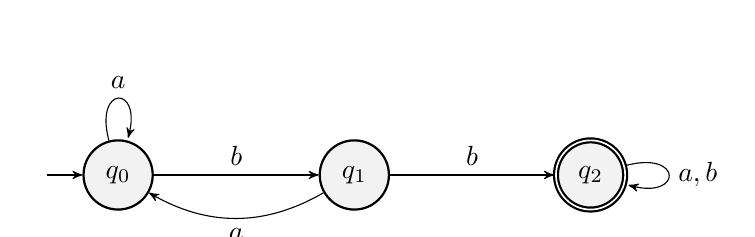
\begin{tikzpicture}
                        \node[state, initial] (q0) {$q_0$};
                        \node[state, right of=q0] (q1) {$q_1$};
                        \node[state, accepting, right of=q1] (q2) {$q_2$};

                        \draw
                        (q0) edge[loop above] node{$a$} (q0)
                        (q0) edge[above] node{$b$} (q1)
                        (q1) edge[above] node{$b$} (q2)
                        (q1) edge[bend left] node[below=0]{$a$} (q0)
                        (q2) edge[loop right] node{$a, b$} (q2);
                    \end{tikzpicture}
                \end{center}
            \end{proof}
            % -------
        \end{enumerate}
    \end{enumerate}

    \newpage
    \fancyhead[c]{Tutorial 6}

    \begin{enumerate}
        \item Let $G$ be the grammar
        \( \begin{aligned}[t]
            S &\to SAB \mid \lambda \\
            A &\to aA \mid a \\
            B &\to bB \mid \lambda 
        \end{aligned} \)
        \begin{enumerate}
            \item Give a leftmost derivation of string $abbaab$.
            \begin{proof}
                $S \to SAB \to SABAB \to ABAB \to aBAB \to abBAB \to abbBAB \to abbAB \to abbaAB \to abbaaB \to abbaabB \to abbaab$
            \end{proof}

            \item Build the derivation tree for the derivations in part (a).
            \begin{proof}
                \leavevmode \par

                \begin{center}
\begin{tikzpicture}[
level distance=1.5cm,
  level 1/.style={sibling distance=5cm},
  level 2/.style={sibling distance=2.5cm},
  level 3/.style={sibling distance=1.5cm},
  every node/.style={circle, draw, minimum size=7mm, inner sep=2pt},
  edge from parent/.style={draw, -latex}
  ]

\node {$S$}
  child {node {$S$}
    child {node {$S$}
        child {node[draw = none] {$\lambda$}}
    }
    child {node {$A$}
        child {node[draw = none] {$a$}}
    }
    child {node {$B$}
        child {node[draw = none] {$b$}}
        child {node {$B$}
            child {node[draw = none] {$b$}}
            child {node {$B$}
                child {node[draw = none] {$\lambda$}}
            }
        }
    }
  }
  child {node {$A$}
    child {node[draw = none] {$a$}}
    child {node {$A$}
        child {node[draw = none] {$a$}}
    }
  }
  child {node {$B$}
    child {node[draw = none] {$b$}}
    child {node {$B$}
        child {node[draw = none] {$\lambda$}}
    }
  };

\end{tikzpicture}
\end{center}
            \end{proof}
            
            \item Generate TWO other possible strings of the language $L(G)$.
            \begin{proof}
            \hfill \\
                1) $aabbab$ \\
                (Derivation: $S \to SAB \to SABAB \to ABAB \to aABAB \to aaBAB \to aabBAB \to aabbBAB \to aabbAB \to aabbaB \to aabbabB \to aabbab$) \\
                
                2) $aaaabb$ \\
                (Derivation: $S \to SAB \to AB \to aAB \to aaAB \to aaaAB \to aaaaB \to aaaabB \to aaaabbB \to aaaabb$)
            \end{proof}
            
            \item Give a regular expression for $L(G)$.
            \begin{proof}
                $L(G)=(aa^*b^*)^*$
            \end{proof}
        \end{enumerate}

        \newpage
        \item 
        \leavevmode \par
        \begin{minipage}{0.30\textwidth}
            \centering
            \begin{tabular}{|c|c|} \hline 
                 No.&  Language\\ \hline 
                 1& 
                $(a+b)^*$\\ \hline
                2&$(a+b)^+$\\\hline
                3&$(a+b)$\\\hline
                4&$(ab)$\\\hline
                5&$a^*bb$\\\hline
                6&$aa^*bb^*$\\\hline
                7&$a^*bba^*$\\\hline
                8&$a(a+b)^*b$\\\hline
                9&$(a+b)^*bb(a+b)^*$\\\hline
                10&$(a+b)^*aa(a+b)^*$\\\hline\end{tabular}
        \end{minipage}
        \hfill
        \begin{minipage}{0.50\textwidth}
            \centering
            \begin{tabular}{|l|l|l|}
                \hline
                Matched No& Grammars&CFG or RG\\
                \hline
                6& \( \begin{aligned}[t]
            S &\to SAB \mid \lambda \\ 
            A &\to aA \mid a \\
            B &\to bB \mid \lambda 
        \end{aligned} \) &CFG\\ \hline 
                5& \( \begin{aligned}[t]
            S &\to Abb \\
            A &\to aA \mid \lambda 
        \end{aligned} \)&CFG\\ \hline
 2& $S \to aS \mid bS \mid a \mid b$&RG\\\hline
 10& \(\begin{aligned}[t]
     S &\to AaaA \\
     S &\to aA \mid bA \mid \lambda
 \end{aligned}\) &CFG\\\hline
 4& \(\begin{aligned}[t]
     S &\to aA \\
     A &\to b
 \end{aligned}\) &RG\\\hline
 9& \(\begin{aligned}[t]
     S &\to aS \mid bS \mid bA \\
     A &\to bB \\
     B &\to aB \mid bB \mid \lambda
 \end{aligned}\) &RG\\\hline
 8& \(\begin{aligned}
     S &\to aA \\
     A &\to aA \mid bA \mid b
 \end{aligned}\) &RG\\\hline
 1& \(S \to aS \mid bS \mid \lambda\) &RG\\\hline
 7& \(\begin{aligned}[t]
     S &\to aS \mid bA \\
     A &\to bB \\
     B &\to aB \mid \lambda
 \end{aligned}\) &RG\\\hline
 3& \(S \to a \mid b\) &RG\\\hline 
                \end{tabular}
        \end{minipage}
    \end{enumerate}


\newpage





\end{document}
